\section{函数的多项式逼近}
\subsection{绪论}
  \begin{defi}[逼近]
    对函数$\f$逼近,即找一简单函数$\g$,使得在某种度量的意义下,
    它们之间的误差最小或足够小.
  \end{defi}

  \begin{thm}[Weierstrass]
    对于定义在$[a, b]$上的连续复函数,存在一列复多项式$\{P_n\}$,
    成立
    \[
      \lim_{n\to\infty}P_n = \f,
    \]
    且是一致的. 若$\f$是实函数,则$P_n$的系数也为实数.
  \end{thm}
  \remark
    Stone-Weierstrass定理
    \footnote{
      \tbf{Theorem(Stone) }
      Suppose $\ms{A}$ is a self-adjoint algebra of complex
      continuous functions on a compact set $K$, $\ms{A}$
      separates points on $K$, and $\ms{A}$ vanishes at no
      point of $K$. Then the uniform closure $\ms{B}$ of
      $\ms{A}$ consists of all complex continuous functions
      on $K$. In other words, $\ms{A}$ is dense in $\ms{C}(K)$.
    }
    保证了至少在最大模的意义下,用多项式
    来逼近函数是可能的.

  \begin{defi}[常用范数]
    对于$\R^n$,常用的范数有
    \begin{enumerate}
      \item $\|\tbf{x}\|_\infty = \max_{1\le i\le n}|x_i|$,
      \item $\|\tbf{x}\|_1 = \sum_{i=1}^n|x_i|$,
      \item $\|\tbf{x}\|_2 = (\sum_{i=1}^nx_i^2)^{1/2}$.
    \end{enumerate}
    对于$\ms{C}[a, b]$,常用的范数有
    \begin{enumerate}
      \item $\|\f\|_\infty = \max_{a\le x\le b}|\f(x)|$,
      \item $\|\f\|_1 = \int_a^b|\f(x)|\rd x$,
      \item $\|\f\|_2 = (\int_a^b\f^2(x) \rd x)^{1/2}$.
    \end{enumerate}
  \end{defi}
  \remark
    通常对于内积空间$X$,可以定义范数为
    \[
      \|\tbf{x}\| = \sqrt{(x, x)}.
    \]

  \begin{defi}[权函数]
    \label{defi: 权函数}
    设$[a,b]$为有限或无限区间\footnote{例子中说$\rho=1$是一个
    常用的权函数,但我没有明白,在无限区间的时候[1.]是如何成立的. }
    ,
    非负函数$\rho(x)$称为$[a,b]$上的权
    函数,若满足
    \begin{enumerate}
      \item $\int_a^b\rho(x)x^k\rd x < \infty$,$k=0,1,2,\dots$,
      \item 对任意非负$\g\in\ms{C}[a, b]$,若$\int_a^b\rho(x)\g(x)\rd x =0$,
      则$g=0$.
    \end{enumerate}
  \end{defi}
  \remark
    利用权函数,可以定义带权内积和范数.

\newpage
\subsection{最佳平方逼近}
  \begin{defi}[最佳平方逼近]
    \label{defi: 最佳平方逼近}
    给定$\f\in\ms{C}[a, b]$和线性无关的函数列$\varphi_0,\dots,
    \varphi_n\in\ms{C}[a, b]$,定义$S_n=\spn\{\varphi_0,
    \dots,\varphi_n\}$,称$\f^*\in S_n$为最佳平方逼近函数,若
    \[
      \|\f^* - \f\| = \min_{\g\in S_n}\|\f-\g\|_2.
    \]
    即$\f^*$是在$2$-范数的含义下,$S_n$中与$\f$最接近的函数.
  \end{defi}
  \remark
    对于离散的情况
    \footnote{
      实际上我们可以利用Riemann-Stieltjes积分定义内积,
      \[\begin{split}
        & (\f,\g) = \int_a^b \f\rd G, \\
        & G(x) =
        \begin{cases}
          \int_a^b\g\rd x,\quad&\text{$\g$为函数,} \\
          \sum_{i=0}^n\f(x_i)I(x-x_i), &\text{$\g$为离散点}
        \end{cases}
      \end{split}\]
      其中$I(x)$为单位阶跃函数. 可以发现,这两种描述的方式是等价的.
      在这样的描述下,对于离散点的$G$实际上是阶梯函数.
    }
    ,可以描述为:给定$x_0,\dots,x_n$处的函数值
    $\f(x_k)$,求$\f^*$,成立
    \[
      \sum_{i=0}^{n}\rho(x_i)|\f(x_j)-\f^*(x_j)|^2 =
      \min_{\g\in S_n}\sum_{i=0}^{n}\rho(x_i)|\f(x_j)-\g(x_j)|^2
    \]

  \begin{thm}[最佳平方逼近的求解]
    设记号同\defref{defi: 最佳平方逼近},设
    \[
      \g(x) = \sum_{i=0}^na_i\varphi_i(x),
    \]
    则可以定义关于$\tbf{a} = (a_0,\dots,a_n)\tr$的函数
    \[\begin{split}
      I(\tbf{a}) = \|\f-\g\|_2^2 &=
      \left\|\f - \sum_{i=0}^na_i\varphi_i\right\|_2^2
      =  \int_a^b \rho\left( \f-\sum_{i=0}^n a_i\varphi_i \right)^2 \rd x.
    \end{split}\]
    根据定义,$I(\tbf{a})$在$\f^*$处取极值,根据Fermat定理,
    在该点各偏导数为零,通常假设$\f$的条件足够好,极限和积分可以换序,即有
    \[\begin{split}
      \frac{\partial I}{\partial a_j} &=
      \int_a^b \frac{\partial}{\partial a_i}
      \rho\left( \f-\sum_{i=0}^n a_i\varphi_i \right)^2 \rd x\\
      &= -2\int_a^b\rho\left( \f-\sum_{i=0}^n a_i\varphi_i \right)\varphi_j \rd x
      = 0.
    \end{split}\]
    即有线性方程组,
    \begin{equation}\begin{cases}
      \label{equ: 法方程}
      (\varphi_0, \varphi_0)a_0 + (\varphi_0, \varphi_1)a_1 + \cdots + (\varphi_0, \varphi_n)a_n = (\f, \varphi_0) \\
      (\varphi_1, \varphi_0)a_0 + (\varphi_1, \varphi_1)a_1 + \cdots + (\varphi_1, \varphi_n)a_n = (\f, \varphi_1) \\
      \dots\dots\\
      (\varphi_n, \varphi_0)a_0 + (\varphi_n, \varphi_1)a_1 + \cdots + (\varphi_n, \varphi_n)a_n = (\f, \varphi_n)
    \end{cases}\end{equation}
    由于$\{\varphi_k\}$线性无关,所以方程组\equref{equ: 法方程}有唯一解.
    设其解为$\tbf{a}^*$,则最佳平方逼近函数即为
    \[
      \f^* = \sum_{i=0}^na^*_i\varphi_i(x),
    \]
  \end{thm}
  \remark
    实际上在计算的时候一般采用Legendre多项式来计算,而非解法方程.
    见\thmref{thm: Legendre多项式的逼近性质}.

  \paragraph{几何描述}
    可以从几何的角度来理解最佳平方逼近. $S_n$是$\{\varphi_k\}$
    张成的空间,而$\f$是$S_n$内或$S_n$外的一个向量,最佳平方逼近
    即找$S_n$中找$\f^*$,使得$\|\f-\f^*\|$最小. 根据几何上的直观,
    $\f-\f^*$应该和$S_n$“垂直”,即与张成$S_n$的向量组中的向量分别
    垂直. 而垂直可以被描述为内积为零. 从而就得到了式\equref{equ: 法方程}.
    (见\figref{fig: 最佳平方逼近几何含义})
    \begin{figure}[htbp]
      \centering
      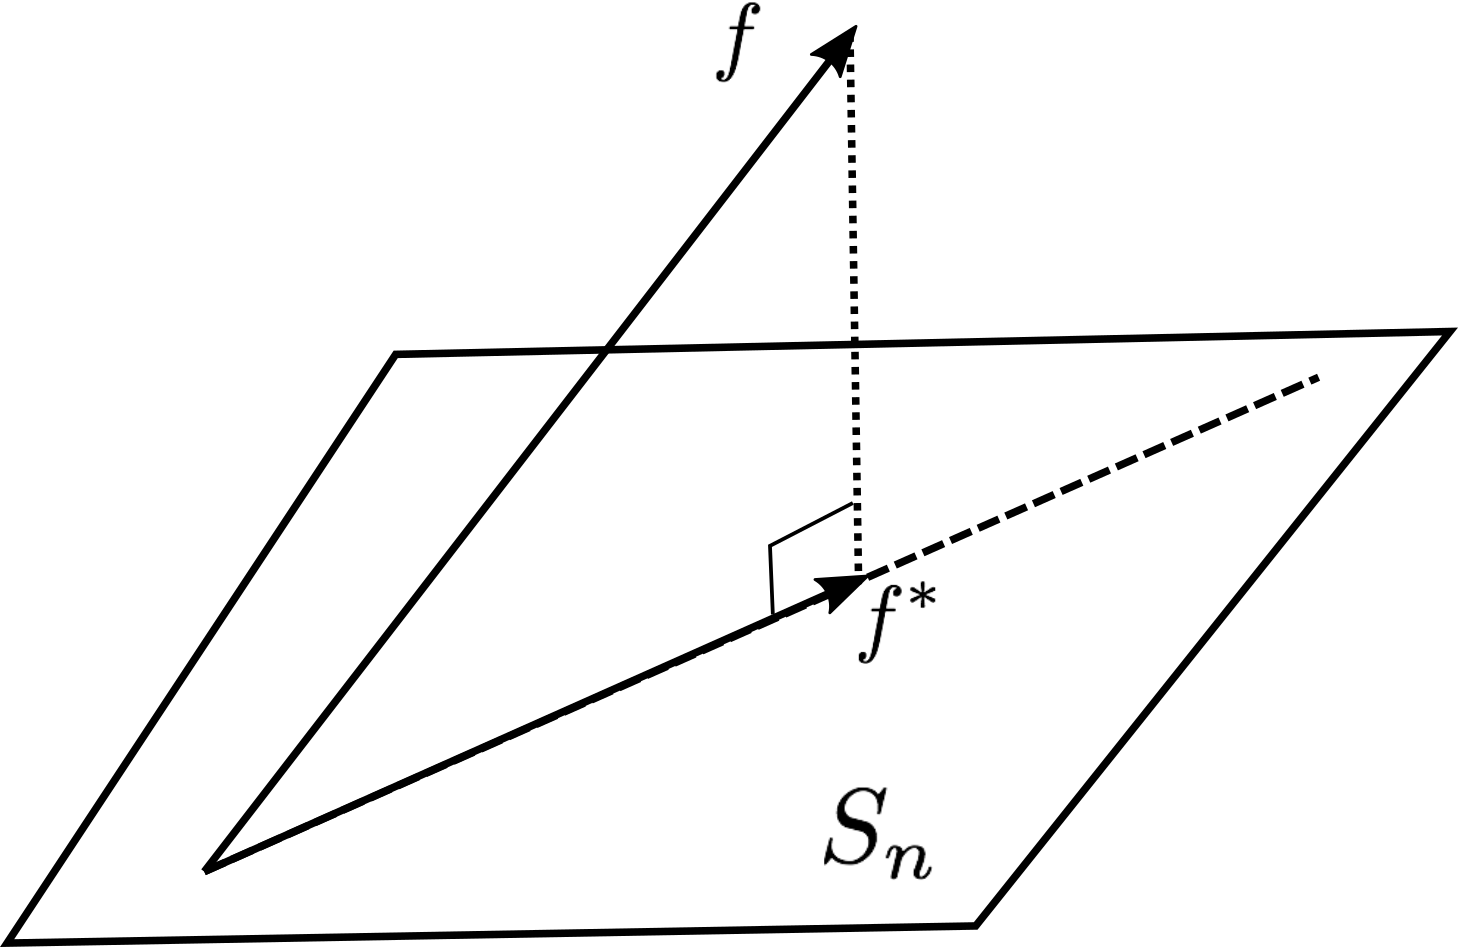
\includegraphics[height=8cm]{../image/least-square.png}
      \caption{最佳平方逼近几何含义}
      \label{fig: 最佳平方逼近几何含义}
    \end{figure}

\newpage
\subsection{正交多项式·绪论}
  \begin{defi}[正交]
    设函数$\f,\g\in\ms{C}[a, b]$,$\rho$为$[a, b]$上的权函数
    且满足
    \[
      (\f, \g) = \int_a^b\rho\f\g\rd x = 0,
    \]
    则称$\f$和$\g$在$[a, b]$上带权$\rho$\tbf{正交}. 若函数组
    $\{\varphi_k\}_{k=0}^\infty$满足
    \[
      (\varphi_i,\varphi_j) =
      \begin{cases}
        0,&\quad i\ne j \\
        A_k>0,& i=j
      \end{cases}
    \]
    则称$\{\varphi_k\}$为$[a, b]$上的带权$\rho$的\tbf{正交函数组}.
    若$A_k=1$,则称为\tbf{标准正交函数组}.
  \end{defi}

  \begin{defi}[正交多项式]
    设$\{\varphi_k\}_{k=0}^\infty$是首项系数$a_n\ne0$的$n$
    次多项式序列. 若它们正交,则称它们为\tbf{正交多项式序列}.
  \end{defi}

  \begin{alg}[Gram-Schmidt正交化]
    设$\{\varphi_k\}$是内积空间$V$的一组基,定义
    \[\begin{split}
      \psi_0 &= \varphi_0, \\
      \psi_{n} &= \varphi_n - \sum_{i=0}^{n-1}(\varphi_n, \psi_i)\eta_i
    \end{split}\]
    其中$\eta_i = \psi_i / \|\psi_i\|^2$. 则$\{\psi_k\}$为
    $V$的一组正交基.
  \end{alg}
  \remark
    要求$n$次正交多项式组,只需另$\varphi_k = x^k$,再进行
    Gram-Schmidt正交化即可.

  \begin{thm}
    设$\{\varphi_n\}_{n=0}^\infty$是一列正交多项式,
    根据正交性(从而线性无关)可以得到正交多项式的如下性质,
    \begin{enumerate}
      \item $P_n \subset \spn\{\varphi_0, \dots,\varphi_n\}$,
      \item 设$P\in P_{n-1}$,则$\varphi_n$与$P$正交.
    \end{enumerate}
  \end{thm}

  \begin{thm}
    设$\{\varphi_n\}_{n=0}^\infty$是$[a,b]$上带权$\rho$的
    正交多项式,则成立
    \[
      \varphi_{n+1} = (x-\alpha_n)\varphi_n - \beta_n\varphi_{n-1},
      \quad n = 0, 1,\dots,
    \]
    其中
    \[\begin{split}
      &\varphi_0 = 1,\quad \varphi_{-1} = 0,\\
      &\alpha_n = (x\varphi_n, \varphi_n) / (\varphi_n, \varphi_n),\\
      &\beta_n = (\varphi_n, \varphi_n) / (\varphi_{n-1}, \varphi_{n-1}).
    \end{split}\]
  \end{thm}
  \proof
    由于齐次性,不妨设$\varphi_n$首项系数为$1$. 所以成立
    \[
      \varphi_{n+1}-x\varphi_n = \sum_{k=0}^n\gamma_k\varphi_k,
    \]
    对于系数$\gamma_k$,成立
    \footnote{
      设$B$是内积空间$V$的一组正交基,则对于任意
      $x\in V$,成立
      \[
        x = \sum_{\beta\in B}\frac{(x,\beta)}{(\beta,\beta)}\beta
      \]
      另外,根据这里内积的定义,成立$(\varphi_i,\varphi_j)
      =(\varphi_i/x, x\varphi_j)$.
    }
    \[
      \gamma_k = \frac{(\varphi_{n+1}-x\varphi_n,\varphi_k)}
      {(\varphi_k, \varphi_k)}
      = \frac{(\varphi_{n+1},\varphi_k) - (\varphi_n, x\varphi_k)}{(\varphi_k,\varphi_k)}.
    \]
    由于$\{\varphi_n\}$正交,所以当$k<n-1$时,成立$\gamma_k=0$.
    所以有
    \[
      \varphi_{n+1} - x\varphi_n = \gamma_n\varphi_n + \gamma_{n-1}\varphi_{n-1}.
    \]
    再进行一些代换,即可以得到原递推式. $\blacksquare$

  \begin{thm}
    设$\{\varphi_n\}_{n=0}^\infty$为$[a, b]$上带权$\rho$的
    正交多项式,则$\varphi_n$在区间$(a, b)$上有$n$个不同的零点.
  \end{thm}
  \proof
    首先利用权函数的定义,证明零点不可能都是偶数重的. 再假设
    $x_1,\dots,x_l$是$\varphi_n$的奇数重零点,则
    \[
      \left(\varphi_n, (x-x_1)\cdots(x-x_l)) \right) \ne 0,
    \]
    再利用正交性可得$l=n$. $\blacksquare$

\newpage
\subsection{Legendre多项式}
  \begin{defi}[Legendre多项式]
    取区间$[-1, 1]$,$\rho(x)\equiv1$,称由$\{1,x,\dots,x^n,\dots\}$
    正交化而得的多项式为Legendre多项式. 其表达式为
    \[
      P_0(x) = 1,\quad
      P_n(x) = \frac{1}{2^nn!}\frac{\rd^n}{\rd x^n}(x^2-1)^n,
      \quad n=1,2,\dots
    \]
    首项系数为$1$的Legendre多项式为
    \[
      \widetilde{P}_n(x) = \frac{n!}{(2n)!}\frac{\rd^n}{\rd x^n}(x^2-1)^n.
    \]
  \end{defi}

  \begin{thm}[Legendre多项式的性质]
    Legendre多项式有如下性质,
    \begin{enumerate}
      \item 正交性:
      \[
        \int_{-1}^1 P_n(x)P_m(x)\rd x =
        \begin{cases}
            0, &\quad m\ne n, \\
            \dfrac{2}{2n+1},&\quad m = n.
        \end{cases}
      \]
      \item 奇偶性:
        \[P_n(x) = (-1)^nP_n(-x),\]
      \item 递推关系:
      \[
        (n+1)P_{n+1} = (2n+1)xP_n - nP_{n-1},\quad
        n = 1, 2,\dots
      \]
    \end{enumerate}
  \end{thm}
  \proof todo

  \begin{thm}[Legendre多项式的逼近性质]
    \label{thm: Legendre多项式的逼近性质}
    在区间$[-1, 1]$上,设$\widetilde{L}_n$是首项系数为$1$的
    Legendre多项式,则
    \[
      \|\widetilde{L}_n\|_2 = \min_{P\in P_n}\|P(x)\|_2.
    \]
  \end{thm}
  \remark
    应用方法和说明可以参考Chebyshev多项式的逼近性质.
    (\thmref{thm: Chebyshev多项式的逼近性质})

  \begin{lemma}[前$4$项Legendre多项式]
    \[\begin{split}
      P_0 &= 1,\\
      P_1 &= x,\\
      P_2 &= \frac{3}{2}x^2 - \frac{1}{2},\\
      P_3 &= \frac{5}{2}x^3 - \frac{3}{2}x
    \end{split}\]
  \end{lemma}

\newpage
\subsection{Chebyshev多项式}
  \begin{defi}[Chebyshev多项式]
    取区间$[-1, 1]$,$\rho(x)=(1-x^2)^{-1/2}$,称由$\{1,x,\dots,x^n,\dots\}$
    正交化而得的多项式为Chebyshev多项式. 其表达式为
    \[
      T_n(x) = \cos(n\arccos x),\quad|x|\le 1
    \]
  \end{defi}

  \begin{thm}[Chebyshev多项式的性质]
    Chebyshev多项式有如下性质,
    \begin{enumerate}
      \item 递推关系:
      \[\begin{split}
        &T_0(x) = 1, \quad T_1(x) = x,\\
        &T_{n+1}(x) = 2xT_n(x) - T_{n-1}(x),\quad n =1,2,\dots
      \end{split}\]
      \item 正交性:
      \[
        \int_{-1}^1\frac{T_n(x)T_m(x)}{\sqrt{1-x^2}} \rd x =
        \begin{cases}
          0, &\quad n\ne m,\\
          \pi/2, &\quad n = m \ne 0,\\
          \pi,&\quad n = m = 0.
        \end{cases}
      \]
      \item $T_{2k}(x)$只含$x$的偶次幂,$T_{2k+1}(x)$只含$x$的
      奇次幂.
      \item $T_n$在区间$[-1, 1]$上的$n$个零点为
      \[
        x_k = \cos\frac{2k-1}{2n}\pi,\quad k = 1,2,\dots,n.
      \]
      \item $T_n$的首项系数为$2^{n-1}$.
    \end{enumerate}
  \end{thm}

  \begin{thm}[Chebyshev多项式的逼近性质]
    \label{thm: Chebyshev多项式的逼近性质}
    在区间$[-1,1]$上,设$\widetilde{T}_n$是首项系数
    为$1$的Chebyshev多项式,则
    \[
      \|\widetilde{T}_n\|_\infty = \min_{P\in\widetilde{P}_n}
      \|P(x)\|_\infty = \frac{1}{2^{n-1}}.
    \]
  \end{thm}
  \remark
    这一定理意味着,取区间$[-1, 1]$,$n$次Chebyshev多项式是所有次数
    小于等于$n$的首项为$1$的多项式中,绝对值的最大值最小的一个. 从而,
    若想用$P_{n-1}$中的多项式来逼近$n$次多项式$\f$,只需找
    $\f^*\in P_{n-1}$,使得
    \[
      \f - \f^* = a_n \widetilde{T}_n.
    \]
    其中$a_n$为$\f$的$n$次项系数. 对于一般的在区间$[a, b]$上的情况,
    只需利用平移和伸缩映射到$[-1, 1]$上即可.

  \begin{thm}[Chebyshev零点插值]
    设插值节点$x_0,\dots,x_n$为Chebyshev多项式$T_{n+1}$的
    零点,被插值函数$\f\in\ms{C}^{n+1}[-1, 1]$,则多项式插值
    的余项$R_n$满足
    \[
      |R_n| \le \frac{1}{2^n(n+1)!}\|\f^{(n+1)}(x)\|_{\infty}.
    \]
  \end{thm}
  \proof
    由于插值点是Chebyshev多项式的零点,所以$\omega_{n+1}=
    \widetilde{T}_n$,所以根据\thmref{thm: Chebyshev多项式的逼近性质},成立
    \[
      \omega_{n+1} \le \frac{1}{2^n}.\quad\blacksquare
    \]
  \remark
    这一定理保证了使用Chebyshev多项式的零点插值,至少可以使得
    误差的最大值最小.
